\documentclass{beamer}
\usetheme{EastLansing}
\usecolortheme{crane}
\usefonttheme{professionalfonts}
\useinnertheme{rectangles}
\usepackage{settings}
%-----------------------------------------------------------------------------%
%%% Title %%%
\title{\textbf{Makefile for Economists}}
\subtitle{An Introduction}
\author{Jesse Chieh Chen}
\date{\texttt{\today}}
%-----------------------------------------------------------------------------%

\begin{document}

\begin{frame}{}
	\maketitle
\end{frame}

\begin{frame}{Road Map}
	\tableofcontents
\end{frame}

\section{The Purpose of Makefile}

\begin{frame}{Economists and their Computers}
	\begin{itemize}
		\item
			What do economists (or a student of economics) do all day with the computer?
			\pause
		\item
			Usually two things:
			\begin{enumerate}
				\item
					Run regression or run simulations.
				\item
					Produce \LaTeX\ (or Beamer) documents.
			\end{enumerate}
		\item
			These tasks are often tied to each other
			and involves several, not difficult, but annoying steps.
	\end{itemize}
\end{frame}

\begin{frame}{Example: Homework}
	\begin{itemize}
		\item
			An assignment requires the following workflow:
			\begin{enumerate}
				\item (R) Run some regression.
				\item (D) Draw some diagram.
				\item (L) Put the regression result and the diagram in the \LaTeX\ document.
				\item (Z) Put the \LaTeX\ pdf and the regression code in a \texttt{zip} and upload it.
			\end{enumerate}
		\item
			Graphically, the workflow looks like this:
	\end{itemize}
	\begin{center}
		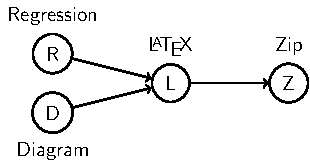
\includegraphics[scale=1]{figures/homework-workflow.pdf}
	\end{center}
\end{frame}

\begin{frame}{The Purpose of \textbf{Makefile}}
	\begin{itemize}
		\item
			A \textbf{Makefile} offers a way to \red{specify and automate} the entire process with a \blue{simple text file}.
		\item
			A \textbf{Makefile} is a text file that specifies a workflow for the program \blue{\texttt{make}}.
		\item
			The program \href{https://www.gnu.org/software/make/}{\blue{\texttt{make}}} is a free and open source GNU project.
		\item
			It is pre-installed on almost all Unix-like systems, including MacOS.
			\begin{itemize}
				\item
					It can be installed on Windows.
			\end{itemize}
		\item
			In the following demonstration, I will focus on Unix-like systems.
	\end{itemize}
\end{frame}

\section{What is the Logical Structure of a Makefile?}

\begin{frame}{How is a Makefile Structured?}
	\begin{itemize}
		\item
			The logic of a Makefile is to specify a \red{target file}, then its \blue{dependencies}.
		\item
			So whenever a dependency is changed, the target file should be regenerated.
		\item
			For example, \texttt{homework.pdf} is dependent on \texttt{homework.tex}.
			So \texttt{homework.pdf} should be recompiled whenever \texttt{homework.tex} is changed.
	\end{itemize}
\end{frame}

\begin{frame}{Example: Homework}
	\begin{center}
		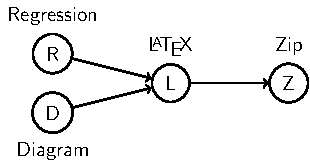
\includegraphics[scale=1]{figures/homework-workflow.pdf}
	\end{center}
	In this example, the dependency structure is as follows:
	\pause
	\begin{itemize}
		\item \red{regression table} depends on the \blue{code 1} and \blue{data} files.
		\item \red{diagram} depends on \blue{code 2}.
		\item \red{\texttt{homework.pdf}} depends on \blue{regressions table}, \blue{diagram}, and \blue{\texttt{homework.tex}}.
		\item \red{\texttt{homework.zip}} depends on \blue{\texttt{homework.pdf}}.
	\end{itemize}
\end{frame}

\section{Praxis}

\subsection{The Shell}

\begin{frame}{A Brief Intro to Shell}
	\begin{itemize}
		\item
			You will need some knowledge about the shell to use Makefiles.
		\item
			When you open a \blue{terminal},
			you are presented with a \blue{shell prompt}.
		\item
			You can traverse the file system and execute commands with the \blue{shell prompt}.
	\end{itemize}
\end{frame}

\begin{frame}{Basic Commands}
	\begin{itemize}
		\item \texttt{pwd}: (print working directory) show where you are currently
		\item \texttt{cd}: (change directory) move to a different directory
			\begin{itemize}
				\item[\texttt{\textbackslash}] root directory
				\item[\texttt{\~}] home directory
				\item[\texttt{.}] current directory
				\item[\texttt{..}] parent directory
			\end{itemize}
		\item \texttt{ls}: (list) list files in the current directory
		\item \texttt{cp}: (copy) copy files or directories
		\item \texttt{mv}: (move) move files or directories
		\item \texttt{rm}: (remove) remove file \red{(CAREFUL! CANNOT UNDO!)}
		\item \texttt{which}: show path of a command
		\item \texttt{clear}: clear the terminal screen
	\end{itemize}
\end{frame}

\begin{frame}{Useful Commands}
	\begin{itemize}
		\item \texttt{pdflatex}: compile \texttt{.tex} file with \texttt{pdflatex} engine.
		\item \texttt{latexmk}: automate \LaTeX\ compilation process
		\item \texttt{R}: interactive R console
		\item \texttt{Rscript}: run R script
		\item \texttt{zip}: make a \texttt{.zip} file
		\item \texttt{make}: to execute a Makefile
	\end{itemize}
\end{frame}

\subsection{Demonstration}

\begin{frame}{Demonstration}
	\begin{itemize}
		\item Example 1: Homework Example.
		\item Example 2: This Beamer Presentation.
		\item Example 3: Beamer Presentation on Chapter 5 of J-SEN.
	\end{itemize}
\end{frame}

\section{Learn More}

\begin{frame}{Resources}
	\begin{itemize}
		\item
			A great resource is a lecture series called \href{https://missing.csail.mit.edu/}{\blue{\texttt{The Missing Semester}}},
			in it a lecture on \href{https://missing.csail.mit.edu/2020/metaprogramming/}{\blue{\texttt{meta-programming}}} also introduces the use of Makefiles.
		\item
			\href{https://missing.csail.mit.edu/}{\blue{\texttt{The Missing Semester}}}
			lecture series introduces a lot of ``workflow'' knowledge that is not typically covered in schools.
		\item
			Here is the \href{https://www.gnu.org/software/make/manual/make.html}{\red{documentation of make}}.
		\item
			You can find the demos of this presentation at \href{https://github.com/jessekelighine/makefile-for-economists}{\texttt{github.com/jessekelighine/makefile-for-economists}}.
	\end{itemize}
\end{frame}

\end{document}
